\documentclass{standalone}
\usepackage{tikz}
\usepackage{calc}
\usepackage{pgffor}
\usetikzlibrary{patterns}
\begin{document}
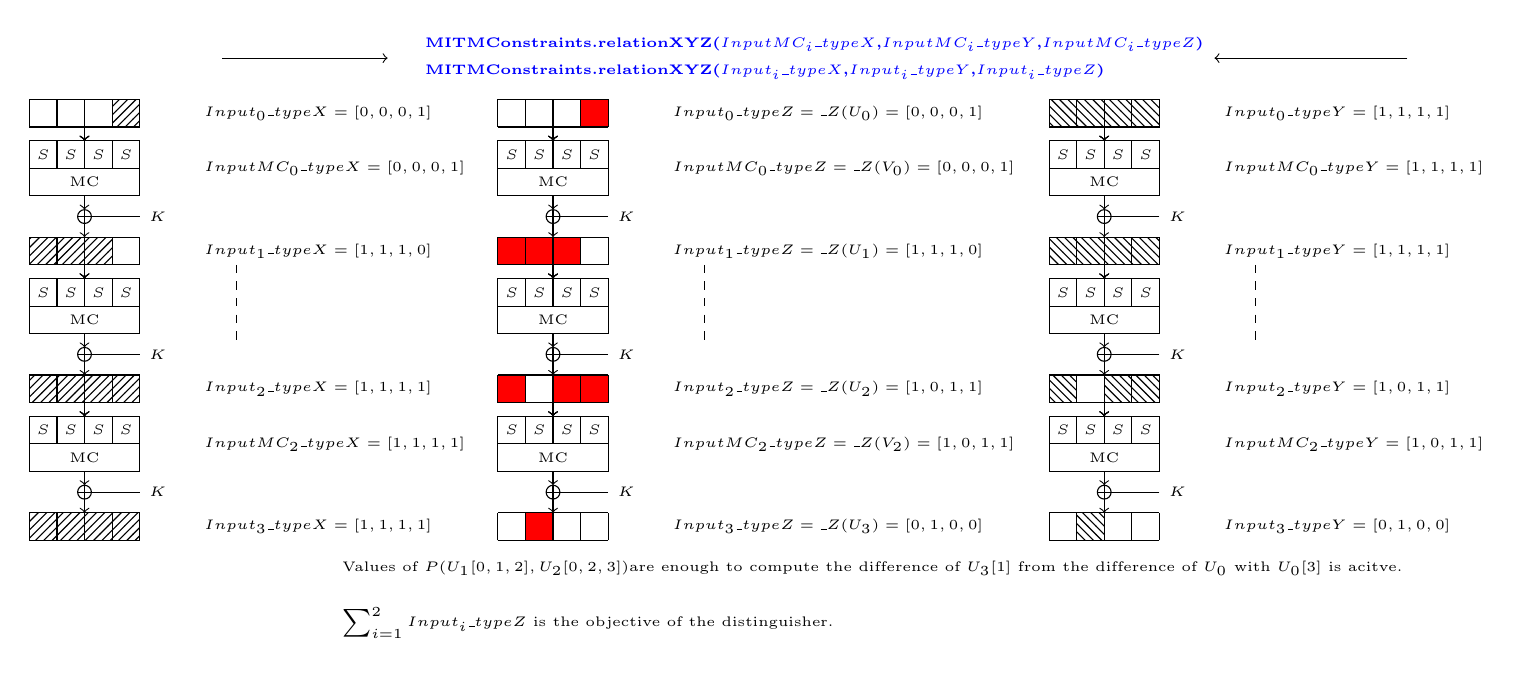
\begin{tikzpicture}[scale=0.35]
\begin{scope}[xshift = -17cm]

\begin{scope}[yshift = 0cm]
\draw[pattern = north east lines](3,0) rectangle+(1,1);

\end{scope}
\begin{scope}[yshift = -5cm]
\draw[pattern = north east lines](0,0) rectangle+(1,1);
\draw[pattern = north east lines](1,0) rectangle+(1,1);
\draw[pattern = north east lines](2,0) rectangle+(1,1);

\end{scope}
\begin{scope}[yshift = -10cm]
\draw[pattern = north east lines](0,0) rectangle+(1,1);
\draw[pattern = north east lines](1,0) rectangle+(1,1);
\draw[pattern = north east lines](2,0) rectangle+(1,1);
\draw[pattern = north east lines](3,0) rectangle+(1,1);

\end{scope}
\begin{scope}[yshift = -15cm]
\draw[pattern = north east lines](0,0) rectangle+(1,1);
\draw[pattern = north east lines](1,0) rectangle+(1,1);
\draw[pattern = north east lines](2,0) rectangle+(1,1);
\draw[pattern = north east lines](3,0) rectangle+(1,1);

\end{scope}
\foreach \z in {0,1,2}{
	\begin{scope}[yshift = -\z* 5 cm]
	\draw (0,0) grid +(4,1);
	\foreach \y in {0,1,2,3}{\draw[->](2,0)--+(0,-0.5);
		\draw(\y,-1.5) rectangle node{\tiny{$S$}} +(1,1);
	}
	\draw (0,-2.5) rectangle node{\tiny{MC}} +(4,1);
	\draw[->] (2,-2.5)--+(0,-0.5);
	\draw (1.75,-3.25)--+(0.5,0);
	\draw (2,-3.25) circle (0.25);
	\draw (4,-3.25) --(2.25,-3.25);
	\node[right] at (4,-3.25) {\tiny{$K$}};
	\draw[->](2,-3)--+(0,-1);
	\end{scope}}

\begin{scope}[yshift = -15 cm]
\draw (0,0) grid +(4,1);
\end{scope}


\begin{scope}[yshift = 0 cm, xshift = 6 cm]
\node[right] at (0, 0.5) {\tiny{$Input_0\_typeX =[0,0,0,1]$}};

%\draw[->] (1.5, 0.3)-- node[right] {\tiny{$SB$}} +(0,-1.5);


\node[right] at (0,-1.5) {\tiny{$InputMC_0\_typeX =[0,0,0,1]$}};

%\draw[->] (1.5, -1.7)-- node[left] {\tiny{$MC$}} +(0,-2.5);
%\node[right] at (1.5,-3) {\tiny{$AK$}};

\node[right] at (0,-4.5) {\tiny{$Input_1\_typeX=[1,1,1,0]$}};

\draw[dashed](1.5,-5) -- +(0,-3);

\end{scope}

\begin{scope}[yshift = -10 cm, xshift = 6 cm]
\node[right] at (0, 0.5) {\tiny{$Input_2\_typeX=[1,1,1,1]$}};

%\draw[->] (1.5, 0.3)-- node[right] {\tiny{$SB$}} +(0,-1.5);


\node[right] at (0,-1.5) {\tiny{$InputMC_2\_typeX=[1,1,1,1]$}};

%\draw[->] (1.5, -1.7)-- node[left] {\tiny{$MC$}} +(0,-2.5);
%\node[right] at (1.5,-3) {\tiny{$AK$}};

\node[right] at (0,-4.5) {\tiny{$Input_3\_typeX=[1,1,1,1]$}};


\end{scope}
\end{scope}



\begin{scope}
%_Z
\begin{scope}[yshift = -5cm]
\fill[red](0,0) rectangle+(1,1);
\fill[red](1,0) rectangle+(1,1);
\fill[red](2,0) rectangle+(1,1);
\end{scope}
\begin{scope}[yshift = -10cm]
\fill[red](0,0) rectangle+(1,1);
\fill[red](2,0) rectangle+(1,1);
\fill[red](3,0) rectangle+(1,1);
\end{scope}
\begin{scope}[yshift = 0cm]
\fill[red](3,0) rectangle+(1,1);
\end{scope}
\begin{scope}[yshift = -15cm]
\fill[red](1,0) rectangle+(1,1);
\end{scope}

\foreach \z in {0,1,2}{
\begin{scope}[yshift = -\z* 5 cm]
\draw (0,0) grid +(4,1);
\foreach \y in {0,1,2,3}{\draw[->](2,0)--+(0,-0.5);
\draw(\y,-1.5) rectangle node{\tiny{$S$}} +(1,1);
}
\draw (0,-2.5) rectangle node{\tiny{MC}} +(4,1);
\draw[->] (2,-2.5)--+(0,-0.5);
\draw (1.75,-3.25)--+(0.5,0);
\draw (2,-3.25) circle (0.25);
\draw (4,-3.25) --(2.25,-3.25);
\node[right] at (4,-3.25) {\tiny{$K$}};
\draw[->](2,-3)--+(0,-1);
\end{scope}}

\begin{scope}[yshift = -15 cm]
\draw (0,0) grid +(4,1);
\end{scope}


\begin{scope}[yshift = 0 cm, xshift = 6 cm]
\node[right] at (0, 0.5) {\tiny{$Input_0\_typeZ = \_Z(U_0)=[0,0,0,1]$}};
\node[right] at(-9,2) {\textbf{\textcolor{blue}{\tiny{MITMConstraints.relationXYZ($Input_i\_typeX$,$Input_i\_typeY$,$Input_i\_typeZ$)}}}};
\node[right] at(-9,3) {\textbf{\textcolor{blue}{\tiny{MITMConstraints.relationXYZ($InputMC_i\_typeX$,$InputMC_i\_typeY$,$InputMC_i\_typeZ$)}}}};
\draw[->] (-16,2.5)--(-10,2.5);
\draw[->] (27,2.5)--(20,2.5);

\node[right] at (0,-1.5) {\tiny{$InputMC_0\_typeZ = \_Z(V_0) =[0,0,0,1]$}};


%\node[right] at (0, -3) {\tiny{MITMConstraints.relationXYZ($InputMC_0\_typeX$,$InputMC_0\_typeY$,$InputMC_0\_typeZ$)}};

\node[right] at (0,-4.5) {\tiny{$Input_1\_typeZ = \_Z(U_1) = [1,1,1,0]$}};

\draw[dashed](1.5,-5) -- +(0,-3);

\end{scope}

\begin{scope}[yshift = -10 cm, xshift = 6 cm]
\node[right] at (0, 0.5) {\tiny{$Input_2\_typeZ= \_Z(U_2) =[1,0,1,1]$}};




\node[right] at (0,-1.5) {\tiny{$InputMC_2\_typeZ = \_Z(V_2) =[1,0,1,1]$}};


%\node[right] at (0, -3) {\tiny{MITMConstraints.relationXYZ($InputMC_2\_typeX$,$InputMC_2\_typeY$,$InputMC_2\_typeZ$)}};

\node[right] at (0,-4.5) {\tiny{$Input_3\_typeZ = \_Z(U_3) = [0,1,0,0]$}};

\end{scope}

\end{scope}



\begin{scope}[xshift = 20cm]
%backward determination
\begin{scope}[yshift = 0cm]
\draw[pattern = north west lines](0,0) rectangle+(1,1);
\draw[pattern = north west lines](1,0) rectangle+(1,1);
\draw[pattern = north west lines](2,0) rectangle+(1,1);
\draw[pattern = north west lines](3,0) rectangle+(1,1);

\end{scope}
\begin{scope}[yshift = -5cm]


\draw[pattern = north west lines](2,0) rectangle+(1,1);
\draw[pattern = north west lines](3,0) rectangle+(1,1);
\draw[pattern = north west lines](0,0) rectangle+(1,1);
\draw[pattern = north west lines](1,0) rectangle+(1,1);
\end{scope}
\begin{scope}[yshift = -10cm]

\draw[pattern = north west lines](3,0) rectangle+(1,1);
\draw[pattern = north west lines](0,0) rectangle+(1,1);
\draw[pattern = north west lines](2,0) rectangle+(1,1);
\end{scope}
\begin{scope}[yshift = -15cm]


\draw[pattern = north west lines](1,0) rectangle+(1,1);
\end{scope}
\foreach \z in {0,1,2}{
	\begin{scope}[yshift = -\z* 5 cm]
	\draw (0,0) grid +(4,1);
	\foreach \y in {0,1,2,3}{\draw[->](2,0)--+(0,-0.5);
		\draw(\y,-1.5) rectangle node{\tiny{$S$}} +(1,1);
	}
	\draw (0,-2.5) rectangle node{\tiny{MC}} +(4,1);
	\draw[->] (2,-2.5)--+(0,-0.5);
	\draw (1.75,-3.25)--+(0.5,0);
	\draw (2,-3.25) circle (0.25);
	\draw (4,-3.25) --(2.25,-3.25);
	\node[right] at (4,-3.25) {\tiny{$K$}};
	\draw[->](2,-3)--+(0,-1);
	\end{scope}}

\begin{scope}[yshift = -15 cm]
\draw (0,0) grid +(4,1);
\end{scope}


\begin{scope}[yshift = 0 cm, xshift = 6 cm]
\node[right] at (0, 0.5) {\tiny{$Input_0\_typeY =[1,1,1,1]$}};

%\draw[->] (1.5, -1.2)-- node[right] {\tiny{$SB$}} +(0,1.5);


\node[right] at (0,-1.5) {\tiny{$InputMC_0\_typeY =[1,1,1,1]$}};

%\draw[->] (1.5, -4.2)-- node[left] {\tiny{$MC$}} +(0,2.5);
%\node[right] at (1.5,-3) {\tiny{$AK$}};


\node[right] at (0,-4.5) {\tiny{$Input_1\_typeY =[1,1,1,1]$}};

\end{scope}

\draw[dashed](7.5,-5) -- +(0,-3);

\begin{scope}[yshift = -10 cm, xshift = 6 cm]
\node[right] at (0, 0.5) {\tiny{$Input_2\_typeY =[1,0,1,1]$}};

%\draw[->] (1.5, -1.2)-- node[right] {\tiny{$SB$}} +(0,1.5);


\node[right] at (0,-1.5) {\tiny{$InputMC_2\_typeY = [1,0,1,1]$}};
%
%\draw[->] (1.5, -4.2)-- node[left] {\tiny{$MC$}} +(0,2.5);
%\node[right] at (1.5,-3) {\tiny{$AK$}};

\node[right] at (0,-4.5) {\tiny{$Input_3\_typeY=[0,1,0,0]$}};

\end{scope}

\end{scope}


\begin{scope}[yshift = -18 cm]
\node[right] at (-6,2) {\tiny{Values of $P(U_1[0,1,2],U_2[0,2,3])$are enough to compute the difference of $U_3[1]$ from the difference of $U_0$ with $U_0[3]$ is acitve.}};

\node[right] at (-6,0) {\tiny{$\sum_{i=1}^{2} Input_i\_typeZ$ is the objective of the distinguisher.}};
\end{scope}
\end{tikzpicture}
\end{document}